% !TeX spellcheck = es_ES
%----------------------------------------------------------------------------------------
%	PACKAGES AND OTHER DOCUMENT CONFIGURATIONS
%----------------------------------------------------------------------------------------

\documentclass[fleqn,10pt]{SelfArx} % Document font size and equations flushed left
%\usepackage{chemmacros}
\usepackage{ifthen}
\usepackage{calc}
\usepackage{microtype}
\usepackage{ifpdf}
\usepackage[utf8]{inputenc}
\usepackage{amsmath, amsfonts, amssymb}
\usepackage{graphicx, xcolor}
\usepackage{booktabs}
\usepackage{fancyhdr}
\usepackage{lastpage}
\usepackage{titlesec}
\usepackage{titletoc}
\usepackage{enumitem}
\usepackage{cuted}
\usepackage[version=3]{mhchem}
\usepackage{lipsum}
\usepackage{graphbox}
\usepackage{cuted}
\usepackage{tabularx}
%----------------------------------------------------------------------------------------
%	COLUMNS
%----------------------------------------------------------------------------------------

\setlength{\columnsep}{0.55cm} % Distance between the two columns of text
\setlength{\fboxrule}{1pt} % Width of the border around the abstract

%----------------------------------------------------------------------------------------
%	COLORS
%----------------------------------------------------------------------------------------

\definecolor{color1}{RGB}{0,94,157} % Color of the article title and sections
\definecolor{color2}{RGB}{255,243,210} % Color of the boxes behind the abstract and headings

%----------------------------------------------------------------------------------------
%	HYPERLINKS
%----------------------------------------------------------------------------------------

\usepackage{hyperref} % Required for hyperlinks
\hypersetup{hidelinks,colorlinks,breaklinks=true,urlcolor=color2,citecolor=color1,linkcolor=color1,bookmarksopen=false,pdftitle={Title},pdfauthor={Author}}

%----------------------------------------------------------------------------------------
%	ARTICLE INFORMATION
%----------------------------------------------------------------------------------------

\JournalInfo{L. de Qu\'imica inorg\'anica II, No. 1, 2016-20} % Journal information
%\Archive{Additional note} % Additional notes (e.g. copyright, DOI, review/research article)

\PaperTitle{Reacci\'on de Cr(III) con un ligando multidentado} % Article title


\Authors{Juan Barbosa{\color{color1}\textsuperscript{1}\textsuperscript{,2}*},
	Alejandro Camacho{\color{color1}\textsuperscript{1}\textsuperscript{,3}**}} %
%Authors
\affiliation{{\color{color1}\textsuperscript{1}}\textit{Departamento de Qu\'imica, Universidad de los Andes, Bogot\'a, Colombia}} % Author affiliation
\affiliation{{\color{color1}\textsuperscript{2}}\textit{Departamento de F\'isica, Universidad de los Andes, Bogot\'a, Colombia}} % Author affiliation
\affiliation{{\color{color1}\textsuperscript{3}}\textit{Departamento de	F\'isica, Universidad Nacional, Bogot\'a, Colombia}}
\affiliation{{\color{color1}*}\textbf{Email}: js.barbosa10@uniandes.edu.co} %
%Corresponding author
\affiliation{{\color{color1}**}\textbf{Email}: a.camacho10@uniandes.edu.co}
\Keywords{ Cinética, orden de reacción, pH, paso determinante de una reacción, Cromo.} %
%Keywords - if you don't want any simply remove all the text between the curly
%brackets
\newcommand{\keywordname}{Keywords} % Defines the keywords heading name

%----------------------------------------------------------------------------------------
%	ABSTRACT
%----------------------------------------------------------------------------------------
\Abstract
{
En la practica se realiza el estudio cinético de la quelación del Cromo (III) con EDTA con el propósito de encontrar la ley de velocidad y sus dependencias para este proceso, partiendo de los supuestos aportados por la la literatura y realizando el análisis de los valores de absorbacia medidos, se encuentra que la velocidad de la reacción depende directamente de la concentración del cromo e inversamente con un orden de $\ce{-0.32 \pm 0.14 }$. Además se entreven aplicaciones del cromo a la hora de estudiar en tiempos reducidos sistemas que dependan en su velocidad del pH de la solución debido a la alta sensibilidad de la estructura de los compuestos de Cromo y EDTA a la concentración de iones $\ce{[H]^{+}}$ y a la alta estabilidad del cromo como ión \ce{Cr^{(III)}}.
}

%----------------------------------------------------------------------------------------

\begin{document}
	\flushbottom % Makes all text pages the same height
	\maketitle % Print the title and abstract box
	%\tableofcontents % Print the contents section
	\thispagestyle{empty} % Removes page numbering from the first page
	%----------------------------------------------------------------------------------------
	%	ARTICLE CONTENTS
	%----------------------------------------------------------------------------------------
	\section*{Introducci\'on}
	El EDTA es un ligando bastante efectivo debido a su estructura \autoref{sch: EDTA} y al efecto quelato, que junto con un precio medio en el mercado permite que tenga múltiples aplicaciones en la industria.
	Un ejemplo de esto es que el EDTA es utilizado como quelante de metales tanto en sangre como en hueso, muy útil en intoxicaciones con plomo, debido a que permite la eliminación del metal y el EDTA puede recuperarse por vía urinaria en un 99\%, garantizando esto su eliminación causando efectos secundarios que desaparecen una vez se retira el tratamiento o aplicando en conjunto con otras sustancias o en forma de sal. También se utiliza como anti-coagulante en muestras de sangre, para ablandar aguas duras en productos de limpieza, como estabilizante y conservante en alimentos.
	\begin{scheme}[h]
	    \centering
	    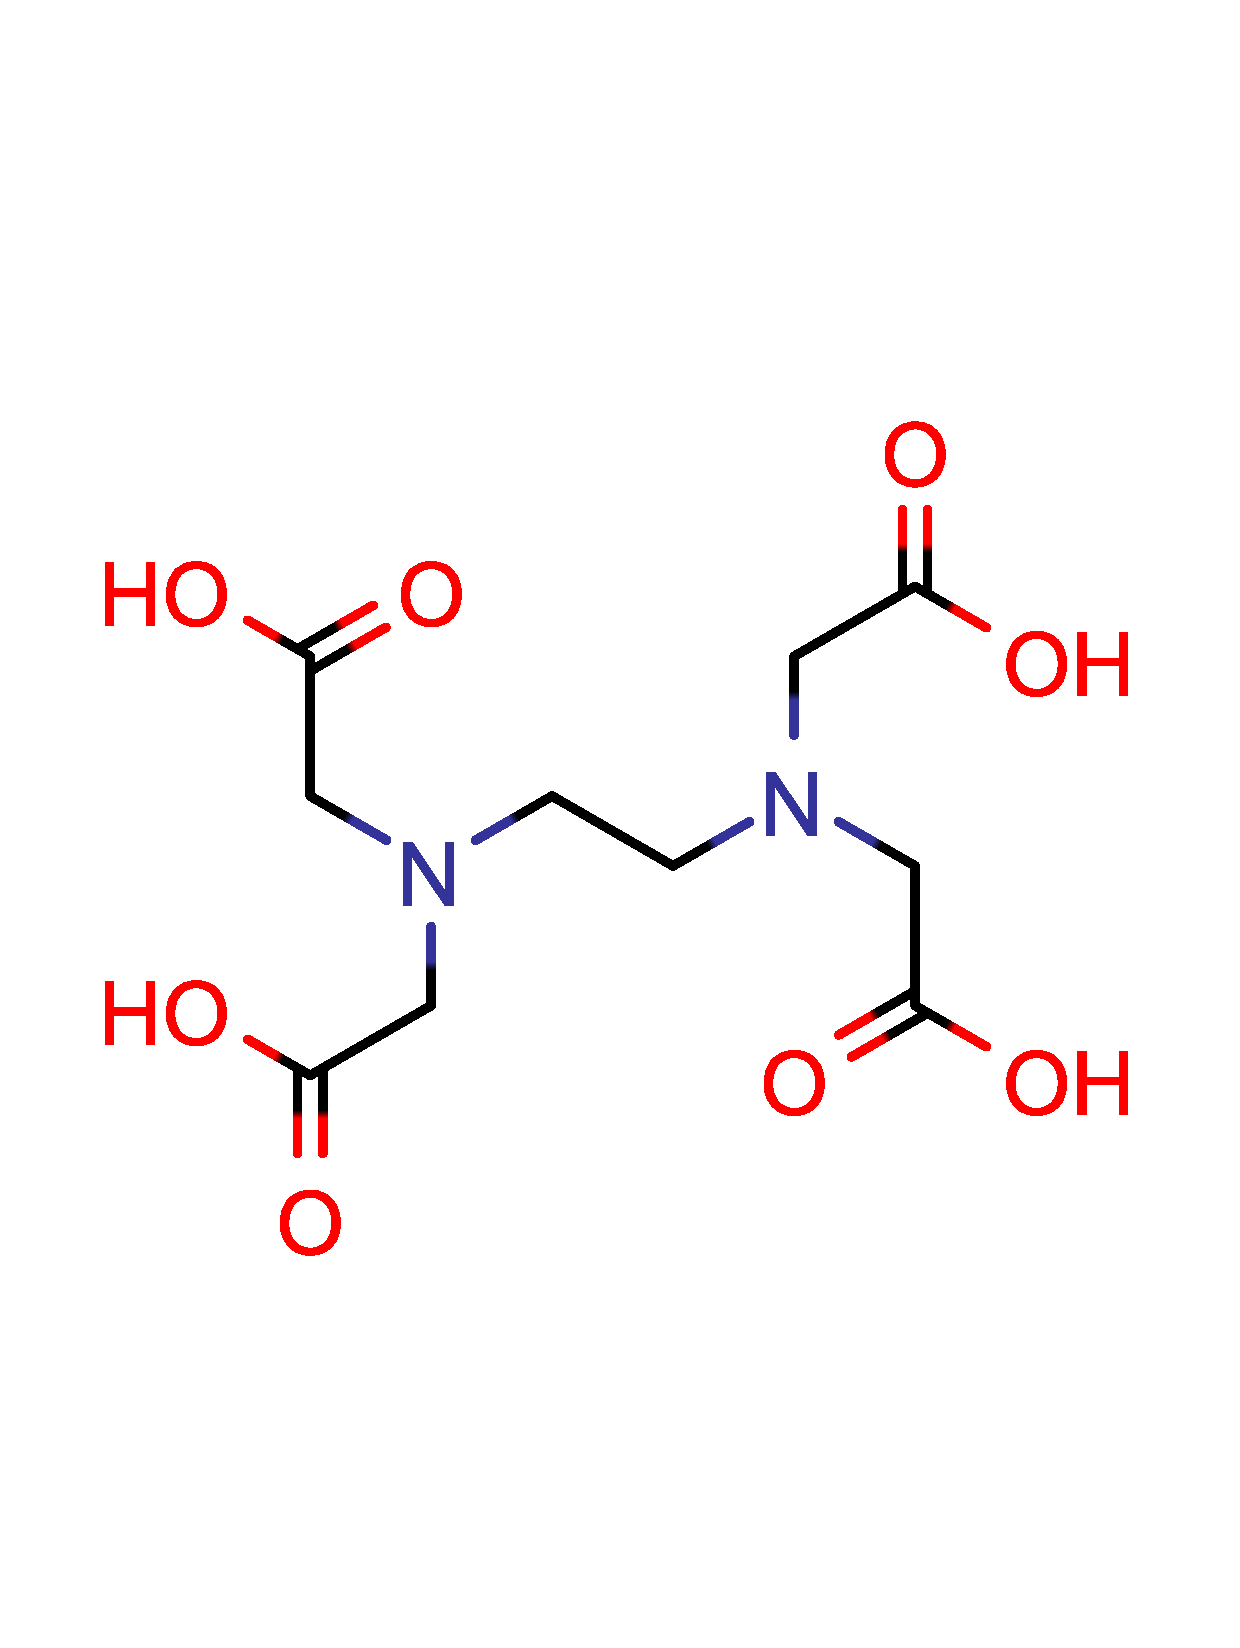
\includegraphics[scale=0.2]{images/EDTA.pdf}
	    \caption{Estructura del EDTA usado en el experimento.}
	    \label{sch: EDTA}
	\end{scheme}
	
	La interacción entre una solución de complejo de Cromo y una solución de EDTA no es una reacción inmediata a temperatura ambiente y pH medio, provocando esto que las propiedades del complejo de Cromo adicionado se mantengan durante un tiempo tornándose la coloración del mismo cada vez mas tenue a medida que es quelado por el EDTA, este proceso ocurre en el transcurso de algunos minutos. Es posible por tanto estudiar la cinética de esta reacción midiendo progresivamente la absorbancia de la muestra y con esto la concentración del producto en formación. En la literatura se encuentra que en esta quelación se presentan numerosos pasos y e intermediarios, sin embargo, es de interés en esta practica el paso determinante de la reacción que permite establecer la constante y la velocidad de la misma. Se espera que el cromo agregado sea completamente quelado por el EDTA debido al exceso del mismo y al considerable aumento de la entropía del sistema. Ocurriendo estereométricamente como se muestra en \autoref{sch: reaccion}.
	\begin{scheme}[h]
	    \centering
	    \ce{Cr^{(III)} + EDTA -> Cr(EDTA) \\}
	   \caption{Reacci\'on de quelación esperada.}
	    \label{sch: reaccion}
	\end{scheme}

	De acuerdo a los estudios realizados por Randall E. Hamm \cite{Hamm} la velocidad del paso determinante de la reacción depende directamente de la concentración del cromo y es inversamente proporcional a la concentración de iones \ce{[H^+]}, así propone \autoref{eq: leyVelocidad}, donde se espera que m sea 1 y que n sea negativo situación a comprobar durante la practica.
	\begin{equation}
	\label{eq: leyVelocidad}
	    \ce{-\dfrac{d\ce{[Cr]}}{dt}=\dfrac{d\ce{[CrEDTA]}}{dt}=k\ce{[Cr]}^m\ce{[H]}^n}
	\end{equation}
	
	\begin{figure*}[!ht]
	    \centering
	    \includegraphics[width=\linewidth]{images/3dplot.pdf}
	    \caption{Progreso de la reacci\'on a pH 3.51.}
	    \label{fig: 3dProgress}
	\end{figure*}

	\section{Metodolog\'ia}
	Se prepara una solución de EDTA (ácido etilendiaminatetraacetato) a una concentración de 0.1 M en la que se varia el pH entre 3.49 y 3.6, sin perder de vista que el EDTA permanezca en solución y que este cambio provocara a su vez que el EDTA tenga mas o menos dientes libres \autoref{fig: EDTAcomposition}. Además se prepara otra solución de tricloruro de cromo hexahidratado $\ce{CrCl_{3}} \cdot \ce{6(H_{2}O)}$ a una concentración de 0.012 M, garantizando así que en la reacción el EDTA sea el reactivo en exceso.
	
	Luego considerando el tiempo de inicio se mezclan 5 mL de cada solución y se realiza este mismo proceso con soluciones de EDTA a diferentes pH, tomando medida de la absorbancia periódicamente para determinar los cambios en la concentración del producto. 

	\section{Resultados y Discusi\'on}
	
	En la \autoref{fig: 3dProgress} se muestra la absorbancia del complejo de cromo con el EDTA en el rango visible a pH 3.51. Las l\'ineas distintas de azul corresponden con los espectros medidos, mientras los azules corresponden con puntos obtenidos usando interpolaci\'on segmentaria c\'ubica. Lo anterior permite predecir el comportamiento en puntos intermedios, completando la informaci\'on ausente. En la misma g\'rafica se puede observar el espectro del complejo en el tiempo $t = \infty$ en verde, con el cual se obtiene la longitud de onda de absorbancia m\'axima. El seguimiento a esta longitud se muestra en la \autoref{fig: Absorbance} con los puntos verdes.
	\begin{figure}[h]
	    \centering
	    \includegraphics[width=\linewidth]{images/Absorbance.pdf}
	    \caption{Progreso de la reacci\'on siguiendo la absorbancia del complejo \ce{Cr[EDTA]} a distintos valores de pH.}
	    \label{fig: Absorbance}
	\end{figure}
	
	La \autoref{eq: leyVelocidad} es una ecuaci\'on diferencial ordinaria de orden $m+n$. Adicionalmente tiene la forma de ecuaci\'on potencial, lo cual supone una ventaja importante a la hora de resolverla, dado que la integral de una potencia es anal\'itica. Es importante notar que la misma se encuentra en funci\'on de la concentraci\'on del cromo libre. Para obtener la concentraci\'on de este en cualquier instante de tiempo resulta necesario aplicar la ley de Beer.
	\begin{equation}
	    \epsilon=\dfrac{A(t)}{C_{\ce{[CrEDTA]}}(t) b}
	\end{equation}
	
	Para $t = \infty$ se espera que todo el cromo (III) inicial se encuentre quelado con el EDTA. Por lo cual la concentraci\'on del complejo CrEDTA en el infinito es igual a la inicial de cromo (III). Reemplazando $b$ por la longitud de la celda, y la absorbancia final se obtiene:
	\begin{table}[h]
	    \centering
	    \caption{Valores del coefficiente absorci\'on molar.}
	    \begin{tabular}{cc}
	        \hline
	        pH & $\epsilon$ (M$^{-1}$cm$^{-1}$)\\
	        \hline
	        3.49 & 515.7 \\
	        3.51 & 433.3 \\
	        4.45 & 412.3 \\
	        4.57 & 389.7 \\
	        5.06 & 492.0 \\
	        5.07 & 418.0 \\
	        5.50 & 420.7 \\
	        5.60 & 420.7 \\
	        \hline
	    \end{tabular}
	    \label{tab: epsilon}
	\end{table}
	\begin{figure*}[!ht]
	    \centering
	    \includegraphics[width=\linewidth]{images/integrationLaws.pdf}
	    \caption{Comportamiento de los diferentes \'ordenes de reacci\'on para el Cr(III) a pH 3.51, los valores marcados con estrellas se encuentran fuera de la tendencia.}
	    \label{fig: integrationLaws}
	\end{figure*}
	
	\pagebreak
	La concentraci\'on en cualquier intante de tiempo de la especie libre de cromo se puede obtener si se tiene en cuenta la conservaci\'on de la masa:
	\begin{equation}
	    C_{\ce{Cr}}(t) = \dfrac{A(\infty)-A(t)}{\epsilon b}
	\end{equation}
	
	Dado que ya se tienen los datos en t\'erminos de la concentraci\'on del \ce{Cr(III)} es posible resolver la \autoref{eq: leyVelocidad} a un pH constante, esto es con $K=k\ce{[H]}^n$.
	\begin{equation}
	    \dfrac{d\ce{[Cr]}}{dt} = -K\ce{[Cr]}^m
	\end{equation}
	
	Separando la ecuaci\'on e integrando a ambos lados:
	\begin{equation}
	    \int\limits_{\ce{[Cr]}_0}^{\ce{[Cr]}}\dfrac{d\ce{[Cr]}}{\ce{[Cr]}^m} = F_m(\ce{[Cr]}) - F_m(\ce{[Cr]}_0) = -K(t-t_0)
	\end{equation}
	
	Dependiendo del valor de $m$ la funci\'on $F_m([C])$ tiene distintas formas. Las tres principales son:
	\begin{equation*}
	    \begin{array}{cc}
	    F_0([C])= & [C] \\
	    F_1([C])= & \ln([C]) \\
	    F_2([C])= & -1/[C] 
	    \end{array}
	\end{equation*}
	
    Usando un algoritmo en Python, de integraci\'on simb\'olica se realiza el ejercicio para $z$ valores arbitrarios de $m$, los cuales en este caso particular oscilan entre $m=-2$ y $m=2$. Los resultados se muestran en la \autoref{fig: integrationLaws}. Existen dos consecuencias importantes que se pueden extraer de la gr\'afica. La primera es que conforme el \'orden de reacci\'on aumenta las funciones adquieren comportamientos asint\'oticos para tiempos prolongados. Lo anterior implica que son propios de reacciones que alcanzan el equilibrio y que no consumen la totalidad de reactivo. Por otro lado los primeros dos valores señalados con estrellas se encuentran fuera de las tendencias. 
    
    Dada la capacidad de quelaci\'on del EDTA y el hecho que este se encuentre en exceso, resulta poco probable que la reacci\'on alcance un equilibrio cuando aun existe cromo libre. Por lo cual el valor de $m$ debe ser $\leq 1$. Por otro lado para los valores menores a $0$ la velocidad de la reacci\'on es inversa a la concentraci\'on del reactivo. Este caso no se observa experimentalmente, apesar que existe una diferencia de dos \'ordenes de magnitud entre la concentraci\'on de EDTA y el cromo.
    
    Por estas razones se restringen los valores de $m$ a mayores que 0 y menores o iguales a 1. En este rango, los menores residuos son alcanzados por $m=1$. Al graficar $F_1([Cr])$ en funci\'on de $t-t_0$ se obtiene una recta cuya pendiente corresponde con $-K$ e intercepto $F_1([Cr]_0)$ como se muestra en la \autoref{fig: logarithmic}.
	\begin{figure}[h]
	    \centering
	    \includegraphics[width=\linewidth]{images/Logarithmic.pdf}
	    \caption{Progreso de la reacci\'on en escala logar\'itmica, siguiendo la concentraci\'on de \ce{Cr(III)}.}
	    \label{fig: logarithmic}
	\end{figure}
	
	Una vez obtenidos los valores de $K$ se puede analizar el efecto del pH. Al aplicar logaritmo sobre $K$ se obtiene:
	\begin{equation}
	    \begin{array}{c}
    	    \log_{10}K=\log_{10}\left(k\ce{[H]}^n\right) \\
    	    \log_{10}K=\log_{10}k - n\text{pH}
	    \end{array}
	\end{equation}
	
	Lo anterior es \'util pues permite obtener el \'orden de reacci\'on frente al hidr\'ogeno y la constante de velocidad, al realizar una gr\'afica del logaritmo de $K$ en funci\'on del pH. Usando la \autoref{fig: pH} se obtiene $n=-0.32\pm0.14$ y $k=(3.4\pm 2.7)\times10^{-6}$ M$^{0.32}$s$^{-1}$, sin tener en cuenta el valor para pH = 3.49, el cual se encuentra fuera de la tendencia. En el caso del hidr\'ogeno coincide con las espectativas para \'ordenes de reacci\'on menores a cero como se observa en la \autoref{fig: integrationLaws}.
	\begin{figure}[h]
	    \centering
	    \includegraphics[width=\linewidth]{images/pH.pdf}
	    \caption{Obtenci\'on del orden de reacci\'on para el hidr\'ogeno.}
	    \label{fig: pH}
	\end{figure}
	
	Adicionalmente se puede predecir el comportamiento del hidr\'ogeno si se tiene en cuenta que la capacidad de quelaci\'on del EDTA depende del n\'umero de dientes que tiene disponibles. En el caso de pH altos el n\'umero de dientes disponible es mayor, dado que los grupos carboxilos tender\'an a estar deprotonados. Lo anterior teniendo en cuenta los valores de pKa del EDTA \cite{Harris}.
	\begin{figure}[h]
	    \centering
	    \includegraphics[width=\linewidth]{images/EDTAcomposition.pdf}
	    \caption{Composici\'on del EDTA seg\'un el pH \cite{Harris}.}
	    \label{fig: EDTAcomposition}
	\end{figure}
	
	Lo anterior se observa f\'acilmente en la \autoref{fig: EDTAcomposition}, en el caso de pH cercano a 3.5, la composici\'on del EDTA oscila entre un 20\% con un \'unico grupo carboxilo deprotonado y 80\% con dos. Mientras que a pH 5.5 el 20\% est\'a compuesto por un \'unico \'acido protonado. Lo cual permite entender la diferencia de velocidades observadas por los compuestos a distintos valores de pH, asi como tambi\'en el orden de reacci\'on obtenido para el hidr\'ogeno. Si bien existe una diferencia considerable entre el orden reportado en la literatura y el obtenido \cite{Hedrick}, se debe tener en cuenta que las mediciones de pH se realizaron en equipos distintos, por lo cual no se pueden tratar como parte del mismo conjunto.
	
	\section{Preguntas}
	\subsection[Derive la ley de velocidad]{Derive la ley de velocidad integrada para una reacci\'on de segundo orden del tipo:}
	\begin{equation}\label{eq: P1}
	    \text{velocidad}=k[A][B]
	\end{equation}
	La ecuaci\'on anterior corresponde a una reacci\'on donde \ce{A + B -> C}, la velocidad se encuentra en t\'erminos de C. Para obtener la ley de velocidad integrada es necesario considerar el progreso de la reacci\'on, esto es que $\ce{[A]} = \ce{[A]_0} - x$ y $\ce{[B]} = \ce{[B]_0}-x$.
	\begin{equation}
	    \dfrac{d\ce{[C]}}{dt}=-\dfrac{d\ce{[A]}}{dt}=-\dfrac{d(\ce{[A]_0} - x)}{dt} = \dfrac{dx}{dt}
	\end{equation}
	
	Aplicando los conceptos anteriores a la \autoref{eq: P1}, separando variables e integrando:
	\begin{equation}
	    \int\limits_{x_0=0}^{x} \dfrac{dx}{(\ce{[A]_0} - x)(\ce{[B]_0} - x)} = k\int\limits_{t_0=0}^{t} dt
	\end{equation}
	
	La parte izquierda se integra usando fracciones parciales, lo cual d
	
	
	
	\begin{equation}
	
	
	    \dfrac{}{}
	    
	\end{equation}
	
	
	
	\normalsize
	
	
	Reemplazando los valores por las concentraciones [A] y [B], y aplicando reglas de logaritmos se obtiene:
	\begin{equation}
	    \dfrac{1}{\ce{[B]_0}-\ce{[A]_0}}\ln\dfrac{\ce{[B][A]_0}}{\ce{[A][B]_0}} = kt
	\end{equation}
	
	\subsection[Cromo (III)]{Cromo (III) es una especie extraordinariamente \'util para la investigaci\'on de la cin\'etica de reacciones. ?`Por qu\'e es tan bueno?}
	El cromo es un elemento altamente reactivo, al existir en al menos seis estados de oxidaci\'on se abre la posibilidad a una gran variedad de estudios. El cromo adem\'as forma complejos estables con distintas esp\'ecies. La composici\'on de los complejos puede ser controlada con el pH, lo cual resulta \'util, dado que es una propiedad sencilla de controlar en soluci\'on \cite{Frost}.
	
	En este estudio en particular el cromo resulta \'util porque en su estado de oxidaci\'on (III) se alcanza el punto de mayor estabilidad, como se muestra en la \autoref{fig: frost}, garantizando que \'este sea la fracci\'on mayoritaria en disoluci\'on.
	\begin{figure}[h]
	    \centering
	    \includegraphics[width=\linewidth]{images/frost.pdf}
	    \caption{Estabilidad de los iones met\'alicos \cite{Frost}.}
	    \label{fig: frost}
	\end{figure}
	
	\subsection[Con respecto]{Con respecto a la pregunta anterior, ?`Por qu\'e el cromo (III) estar\'ia mala elecci\'on?}
	El cromo se encuentra clasificado como metal pesado, raz\'on por la cual deben tomarse precauciones especiales en su manipulaci\'on, lo cual de una u otra manera restringe su uso \cite{Frost}.
	
	\section{Conclusiones}
	Usando un algoritmo de integraci\'on simb\'olica fue posible realizar una simulaci\'on para posibles leyes integradas de velocidad con \'ordenes poco comunes. A partir de esto y la informaci\'on experimental fue posible concluir que el orden de reacci\'on respecto al cromo es 1.
	
	La determinaci\'on del orden de reacci\'on para el hidr\'ogeno se obtiene luego de analizar los datos obtenidos por distintos grupos del laboratorio. Dando un valor de $-0.32\pm0.14$. La constante de velocidad se determina en $(3.4\pm 2.7)\times10^{-6}$ M$^{0.32}$s$^{-1}$.
	\phantomsection
	\bibliographystyle{unsrt}
	\begin{thebibliography}{9}
	    \bibitem{Hamm}
		Hamm E. The Ethylenediaminetetraacetic Acid Complex with Chromium (III). \textit{J Am Chem Soc}. 1953;609(4):5670–2. 
		\bibitem{Harris}
		Harris, D. C. \texit{Quantitative chemical analysis}, 8th ed.; Freeman, W. H. & Company: New York, 2010.
		\bibitem{Hedrick}
		Hedrick, C. E. Formation of the chromium-EDTA complex: An undergraduate kinetics experiment. \textit{Journal of Chemical Education}. DOI: 10.1021/ed042p479. Published Online: Sept 1965, \textit{42} (9), 479.
		\bibitem{Frost}
		Mousavi, Z.; Hosseinifar, A.; Jahed, V. Studies of adsorption thermodynamics and kinetics of Cr(III) and Ni(II) removal by polyacrylamide. \textit{Journal of the Serbian Chemical Society}. DOI: 10.2298/jsc110410172m. Published Online: 2012, 77 (3), 393–405.
		 
	\end{thebibliography}
\end{document}
